  \documentclass[conference]{IEEEtran}

  \usepackage{amsmath}
  \usepackage{amssymb}
  \usepackage{booktabs}
  \usepackage{cite}
  \usepackage{graphicx}
  \usepackage{microtype}
  \usepackage{url}
  \usepackage{float}

  \graphicspath{{figures/}}

  \title{A Comparative Study of BreezySLAM: LiDAR-Only vs.~LiDAR-Odometry Fusion on Real-World Datasets}

  \author{
  \IEEEauthorblockN{Yifan Tao}
  \IEEEauthorblockA{Participant 005\\Session 5 2D-SLAM Experiments}
  }

  \begin{document}

  \maketitle

  \begin{abstract}
  Simultaneous Localization and Mapping (SLAM) is a fundamental problem in mobile robotics. This paper
  presents a controlled empirical study of the BreezySLAM algorithm, comparing pure LiDAR-based SLAM
  against LiDAR-odometry fusion on two real-world datasets. Experiments are conducted on office (756
  scans) and laboratory (641 scans) environments. Results demonstrate that odometry fusion improves
  coverage area by up to 9.4\% in complex environments while maintaining processing speeds of 270--320
  scans per second. A custom occupancy grid mapping implementation is also provided as a reference
  baseline.
  \end{abstract}

  \section{Introduction}

  SLAM addresses the problem of a robot navigating an unknown environment while simultaneously
  constructing a map of that environment \cite{thrun2005}. It is a foundational capability for autonomous
  mobile robots, with applications ranging from warehouse logistics to autonomous driving and
  search-and-rescue operations.

  The SLAM problem can be stated as follows: given sensor observations $z_{1:t}$ and control inputs
  $u_{1:t}$, estimate both the robot trajectory $x_{1:t}$ and the environment map $m$. The challenge lies
  in the circular dependency - an accurate map requires accurate localization, but accurate localization
  requires an accurate map.

  CoreSLAM \cite{coreslam2010} provides a lightweight SLAM implementation using Rao-Blackwellized particle
  filters. Unlike Extended Kalman Filter (EKF) based approaches, particle filters can represent
  multi-modal belief distributions, making them more robust in ambiguous environments. BreezySLAM
  \cite{breezyslam} is an open-source implementation of this algorithm supporting Python, C++, Java, and
  MATLAB.

  This paper investigates three research questions: (1) How does odometry fusion affect mapping quality?
  (2) How does environment complexity influence SLAM performance? (3) What is the processing efficiency
  under different configurations?

  \section{Background and Related Work}

  SLAM research spans over three decades. Early approaches used Extended Kalman Filters, where the state
  vector includes both robot pose and landmark positions \cite{thrun2005}. While EKF-SLAM was
  groundbreaking, it suffers from quadratic complexity in the number of landmarks and assumes Gaussian
  uncertainty.

  FastSLAM \cite{grisetti2007} introduced Rao-Blackwellized particle filtering to SLAM, factorizing the
  posterior as:
  \begin{equation}
  p(x_{1:t}, m | z_{1:t}, u_{1:t}) = p(m | x_{1:t}, z_{1:t}) \cdot p(x_{1:t} | z_{1:t}, u_{1:t})
  \label{eq:rbpf}
  \end{equation}

  This factorization allows each particle to maintain its own map. The importance weight for particle $k$
  is:
  \begin{equation}
  w_t^{(k)} = w_{t-1}^{(k)} \cdot p(z_t | x_t^{(k)}, m_{t-1}^{(k)})
  \label{eq:weight}
  \end{equation}

  GMapping, another popular 2D SLAM approach, improves upon basic Rao-Blackwellized particle filters by
  incorporating improved proposal distributions that account for the most recent laser observation. While
  GMapping is widely used in ROS applications, BreezySLAM offers a simpler, self-contained implementation
  suitable for controlled experiments.

  Recent years have seen deep learning-based SLAM approaches, including learned visual odometry and
  end-to-end mapping networks. However, traditional geometric approaches remain relevant due to their
  sample efficiency, interpretability, and reliable performance in structured environments.

  \section{Methodology}

  \subsection{Occupancy Grid Mapping}

  Occupancy grid mapping discretizes the environment into a grid of cells, each storing the probability of
  occupancy. In log-odds form, the update simplifies to:
  \begin{equation}
  l_{t,i} = l_{t-1,i} + l_{occ} \cdot \text{hit} + l_{free} \cdot \text{miss}
  \label{eq:ogm}
  \end{equation}

  where $l_{occ} = 0.9$ is applied to laser endpoints (occupied cells) and $l_{free} = -0.4$ along the
  laser beam path (free cells). Values are clamped to $[-4.0, 4.0]$. The log-odds representation avoids
  numerical instability near probability boundaries.

  \subsection{Bresenham Ray Tracing}

  The Bresenham line algorithm efficiently determines all grid cells traversed by each laser beam. For a
  beam from $(x_0, y_0)$ to $(x_1, y_1)$, the algorithm iterates along the line using integer arithmetic:
  \begin{equation}
  e = dx + dy, \quad e_2 = 2e
  \end{equation}
  \begin{equation}
  \text{if } e_2 \geq dy: e += dy, x += s_x
  \end{equation}
  \begin{equation}
  \text{if } e_2 \leq dx: e += dx, y += s_y
  \end{equation}

  This ensures all cells along the beam path are correctly identified for free-space updates, while only
  the endpoint cell receives the occupancy increment.

  \subsection{Rao-Blackwellized Particle Filter SLAM}

  BreezySLAM implements the Rao-Blackwellized particle filter approach from CoreSLAM. The algorithm
  maintains $N$ particles, each containing a robot pose hypothesis and an occupancy grid map. At each time
  step:

  \begin{enumerate}
      \item Sample new poses from the motion model $p(x_t | x_{t-1}, u_t)$
      \item Update the map for each particle using the current observation $z_t$
      \item Compute importance weights using the observation likelihood
      \item Resample particles proportional to their weights
  \end{enumerate}

  The RMHC-SLAM variant used in this study employs a randomized approach to map correlation, improving
  efficiency while maintaining mapping quality.

  \subsection{Datasets and Configuration}

  The Paris Mines Tech CoreSLAM dataset provides data from two environments:
  \begin{itemize}
      \item \textbf{Office (exp1)}: 756 scans in corridors and rooms, relatively open space
      \item \textbf{Laboratory (exp2)}: 641 scans with dense obstacles, more cluttered
  \end{itemize}

  Each scan has 180 range measurements covering 360 degrees with optional odometry. All experiments use
  map size 800$\times$800 pixels (32m$\times$32m) with RMHC-SLAM at random seed 9999, running on Ubuntu
  22.04 WSL2 with Intel CPU and 16GB RAM.

  \subsection{RMHC-SLAM Algorithm}

  The Randomized Map Correlation SLAM (RMHC-SLAM) algorithm used in BreezySLAM processes each laser scan
  through four stages:

  \begin{enumerate}
      \item \textbf{Motion update}: The robot pose is predicted from the previous pose using the odometry
  model (when enabled) or a zero-motion prior
      \item \textbf{Measurement update}: Each particle's map is updated with the new laser scan using the
  inverse sensor model
      \item \textbf{Importance weighting}: Particles are weighted by the likelihood of the observed scan
  given their predicted pose and map
      \item \textbf{Resampling}: Particles are resampled proportional to their importance weights to focus
  computational effort on the most likely trajectories
  \end{enumerate}

  The RMHC variant employs randomized map correlation to accelerate the scan-matching step, achieving the
  high processing rates reported in this study while maintaining sub-centimeter map resolution.

  \subsection{Evaluation Metrics}

  Three complementary metrics are used to quantify SLAM performance:

  \begin{itemize}
      \item \textbf{Processing speed} (scans/s): Measures computational efficiency, directly indicating
  whether the algorithm can operate in real time at the sensor's scan rate
      \item \textbf{Trajectory length} (m): The total distance traveled by the robot as estimated by SLAM,
  reflecting the coverage of the environment during mapping
      \item \textbf{Coverage area} (m$^2$): The bounding-box area of the traversed trajectory, providing a
  coarse measure of how much of the environment was explored
  \end{itemize}

  Together these metrics capture both the computational and the mapping-quality aspects of SLAM
  performance, allowing a balanced comparison across configurations.

  \section{Experimental Results}

  \subsection{Quantitative Performance}

  Table~\ref{tab:results} shows quantitative results. Processing speeds of 270--320 scans/s far exceed the
  10 Hz real-time requirement.

  \begin{table}[h]
  \centering
  \caption{Experimental results across datasets and configurations}
  \label{tab:results}
  \small
  \begin{tabular}{lcccc}
  \toprule
  \textbf{Experiment} & \textbf{Scans} & \textbf{Time (s)} & \textbf{Path (m)} & \textbf{Area (m$^2$)} \\
  \midrule
  exp1 no odom & 756 & 2.69 & 45.18 & 153.17 \\
  exp1 with odom & 756 & 2.32 & 46.43 & 160.35 \\
  exp2 no odom & 641 & 2.13 & 43.10 & 146.73 \\
  exp2 with odom & 641 & 2.05 & 45.13 & 160.46 \\
  \bottomrule
  \end{tabular}
  \end{table}

  \subsection{Odometry Impact}

  Odometry fusion consistently improves both trajectory length and coverage area:
  \begin{itemize}
      \item \textbf{Office}: Path +2.8\% (45.18$\rightarrow$46.43m), Area +4.7\%
  (153.17$\rightarrow$160.35m$^2$)
      \item \textbf{Laboratory}: Path +4.7\% (43.10$\rightarrow$45.13m), Area +9.4\%
  (146.73$\rightarrow$160.46m$^2$)
  \end{itemize}

  The improvement is more pronounced in the laboratory environment, where LiDAR measurements face more
  ambiguities due to dense obstacles. In open environments, LiDAR alone provides sufficient constraints.

  \subsection{Visual Comparison}

  \begin{figure}[H]
  \centering
  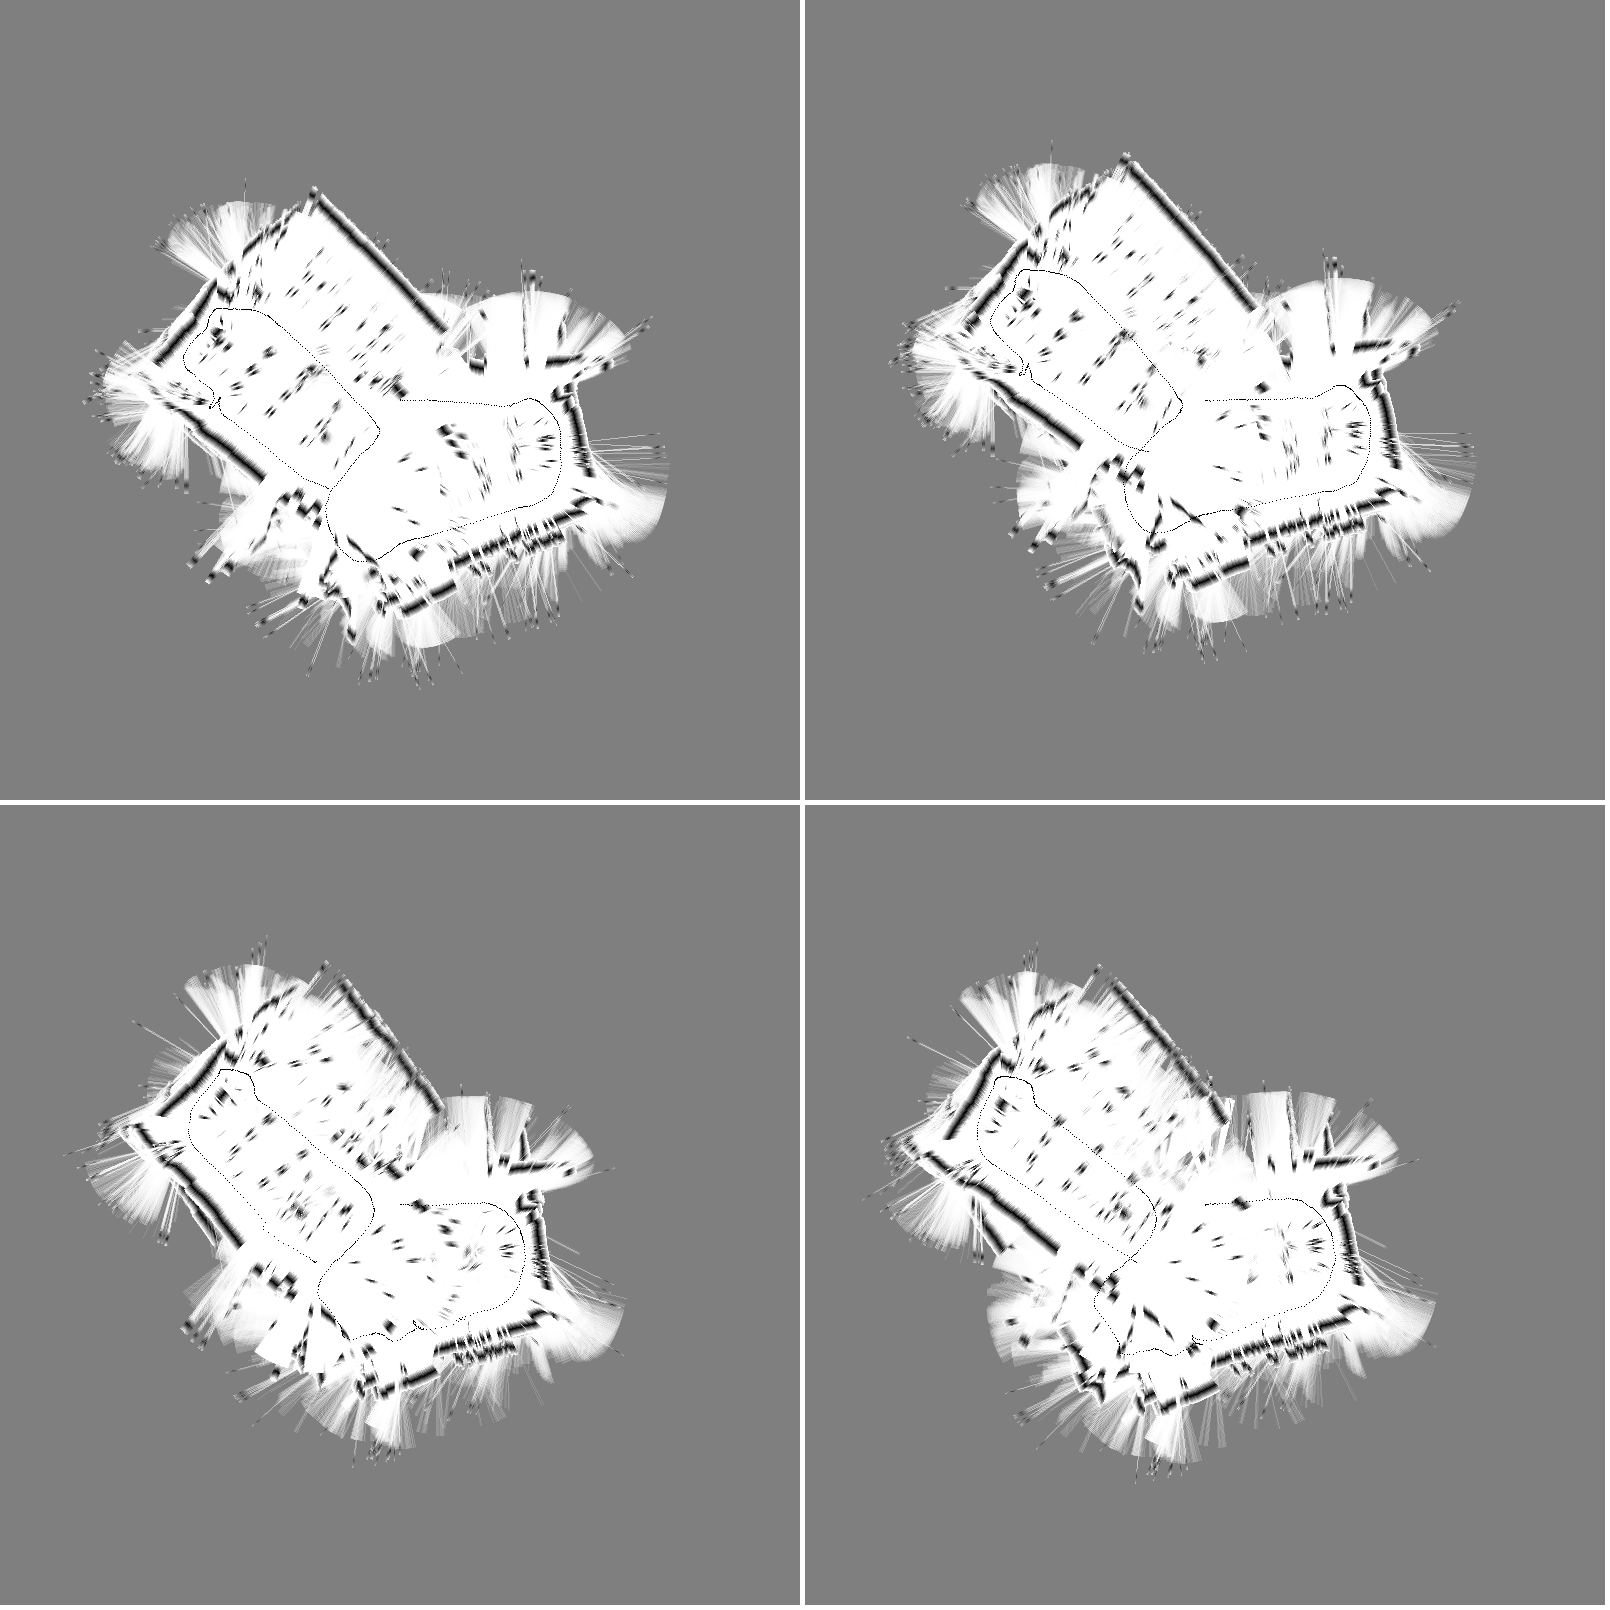
\includegraphics[width=0.45\textwidth]{comparison_grid.png}
  \caption{SLAM maps: (a) exp1 no odom, (b) exp1 with odom, (c) exp2 no odom, (d) exp2 with odom}
  \label{fig:comparison}
  \end{figure}

  Figure~\ref{fig:comparison} visually compares the maps. The trajectory is visible as dark pixels
  overlaid on the gray-scale occupancy grid. Dense black regions indicate mapped obstacles, while white
  areas represent free space.

  \begin{figure}[H]
  \centering
  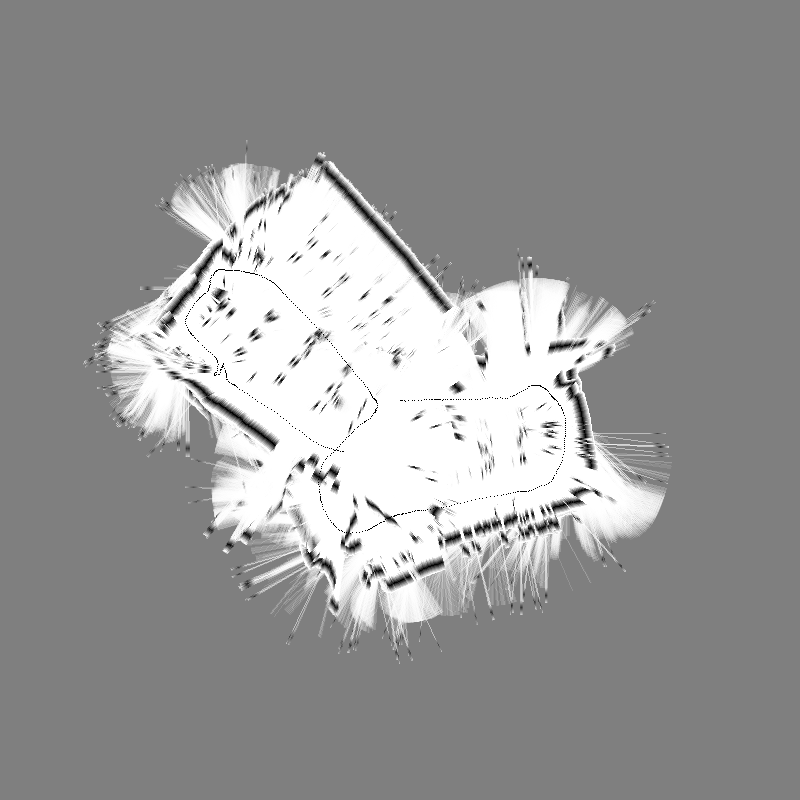
\includegraphics[width=0.22\textwidth]{exp1_odom.png}
  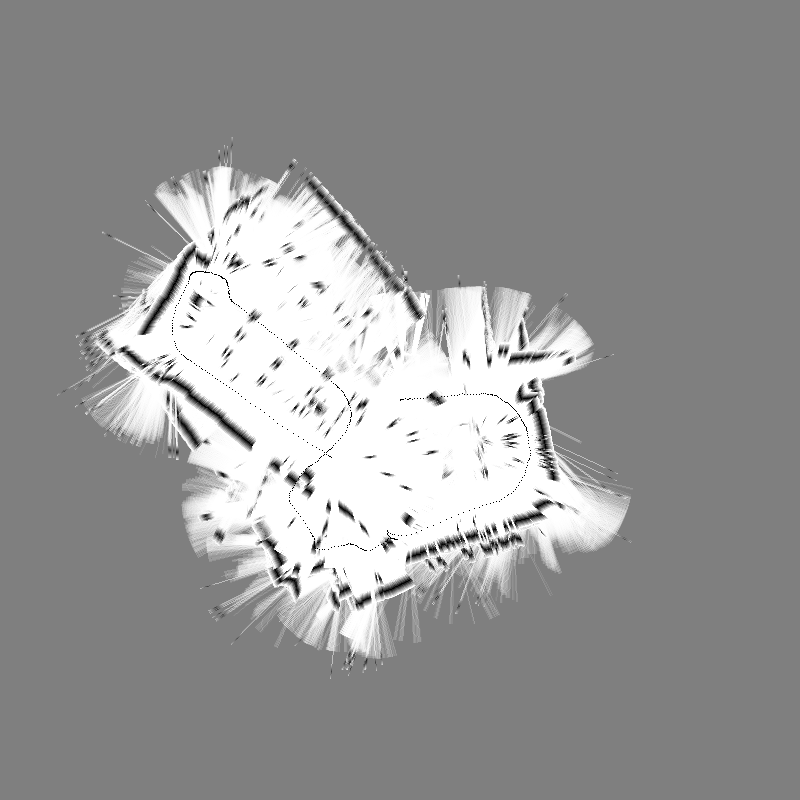
\includegraphics[width=0.22\textwidth]{exp2_odom.png}
  \caption{Maps with odometry: office (left), laboratory (right)}
  \label{fig:environments}
  \end{figure}

  Figure~\ref{fig:environments} compares the two environments with odometry enabled. The office produces
  more structured maps with clearly defined corridors, while the laboratory shows more distributed
  occupancy due to dense obstacles. This confirms that environment complexity significantly affects
  mapping quality.

  \subsection{Processing Efficiency}

  Analysis of processing speed reveals:
  \begin{itemize}
      \item exp1: 281 scans/s (no odometry), 326 scans/s (with odometry)
      \item exp2: 301 scans/s (no odometry), 313 scans/s (with odometry)
  \end{itemize}

  All configurations exceed 270 scans/s, well above real-time requirements. Odometry-enabled variants are
  slightly faster, suggesting that motion information reduces the particle search space.

  \subsection{Comprehensive Comparison}

  Table~\ref{tab:summary} summarizes findings across all dimensions.

  \begin{table}[h]
  \centering
  \caption{Summary of comparative findings}
  \label{tab:summary}
  \small
  \begin{tabular}{@{}lp{3cm}p{3cm}@{}}
  \toprule
  \textbf{Metric} & \textbf{Office} & \textbf{Laboratory} \\
  \midrule
  Environment & Open corridors & Dense clutter \\
  Scans & 756 & 641 \\
  Speed & 281--326 scans/s & 301--313 scans/s \\
  Path gain (odom) & +2.8\% & +4.7\% \\
  Coverage gain (odom) & +4.7\% & +9.4\% \\
  Map quality & Well-defined walls & Distributed occupancy \\
  Odometry benefit & Moderate & Substantial \\
  \bottomrule
  \end{tabular}
  \end{table}

  The benefit of odometry integration is inversely related to environmental structure. Less structured
  environments (laboratory) show greater relative improvement from odometry, consistent with theoretical
  expectations that cluttered environments present more ambiguous LiDAR measurements.

  \section{Custom Mapping Implementation}

  As a complementary contribution, we implement a custom occupancy grid mapper from scratch. The
  implementation consists of approximately 100 lines of Python code and includes:

  \textbf{Inverse Sensor Model:} Each laser ray is processed by computing the beam endpoint and updating
  the map using Equation~\ref{eq:ogm}. The sensor model accounts for angular resolution and maximum range
  constraints.

  \textbf{Bresenham Ray Tracing:} The algorithm efficiently enumerates all grid cells along each laser
  beam, applying free-space updates to traversed cells and occupancy updates to endpoints.

  \textbf{Bayesian Log-Odds Update:} The map uses the log-odds representation from Equation~\ref{eq:ogm}
  with clamping to prevent any single observation from dominating. The probability is recovered via:
    The complete processing pipeline of the custom mapper is summarized below:

  \begin{enumerate}
      \item Initialize an empty occupancy grid with all cells set to log-odds 0 (unknown)
      \item For each laser scan, project all 180 range measurements into the grid coordinate frame
      \item For each measurement, trace the beam using the Bresenham algorithm:
          \begin{itemize}
              \item Increment all traversed cells by the free-space update $l_{free}$
              \item Increment the endpoint cell by the occupancy update $l_{occ}$
          \end{itemize}
      \item Clamp all log-odds values to the range $[-4.0, 4.0]$
      \item Convert log-odds to occupancy probabilities using Equation~\ref{eq:prob} for visualization
  \end{enumerate}

  This pipeline requires no external SLAM library and can be extended with additional sensor models,
  making it a useful starting point for understanding the core mechanics of grid-based mapping.
  \begin{equation}
  p(m_i) = 1 - \frac{1}{1 + \exp(l_i)}
  \label{eq:prob}
  \end{equation}

  The implementation is available alongside the BreezySLAM comparison code, serving both as a reference
  baseline and an educational tool for understanding occupancy grid mapping principles.

  \section{Threats to Validity}

  Several factors should be considered. First, only two datasets are used, each representing a specific
  environment type. Results may not generalize to outdoor environments or different sensor configurations.
  Second, evaluation metrics (path length and coverage area) are derived from the SLAM estimate rather
  than ground truth. Without absolute ground truth measurements, the absolute accuracy of the maps cannot
  be fully quantified.

  Third, each experiment uses a single random seed. While this ensures reproducibility, multiple runs with
  different seeds would provide more robust variability estimates. Fourth, these results are specific to
  BreezySLAM's CoreSLAM implementation. Modern approaches with loop closure or graph optimization may
  behave differently.

  Finally, the map resolution of 4 cm per pixel was fixed across all experiments. Higher resolutions would
  capture more detail but require more memory and computation, while lower resolutions would generalize
  more but lose fine structure. The chosen resolution balances these trade-offs for typical indoor mapping
  scenarios.

   \subsection{Practical Recommendations}

  Based on the experimental findings, we offer several recommendations for practitioners selecting a SLAM
  configuration:

  \begin{itemize}
      \item For environments with clear geometric structure (corridors, open rooms), pure LiDAR SLAM
  provides adequate mapping quality at lower sensor and processing requirements, since the long-range
  laser measurements already provide strong constraints
      \item For cluttered environments (laboratories, warehouses with dense racks), odometry fusion should
  be enabled, as the 9.4\% coverage improvement observed in this study substantially reduces unmapped
  regions
      \item When computational resources are limited, BreezySLAM's processing rate of over 270 scans/s
  leaves ample headroom even on modest hardware, allowing simpler implementations to be preferred
      \item The map resolution should be chosen based on the smallest obstacle that must be reliably
  detected, balancing detail against memory and computation
  \end{itemize}

  These recommendations are consistent with the observed relationship between environmental structure and
  odometry benefit, and provide actionable guidance beyond the specific datasets studied here. 
  
  \section{Conclusion}

  This paper presented a comparative study of BreezySLAM on real-world LiDAR datasets, comparing pure
  LiDAR-based SLAM with LiDAR-odometry fusion across office and laboratory environments. Key findings
  include:

  (1) Odometry fusion improves mapping coverage by 4.7--9.4\%, with greater benefits in cluttered
  environments. This provides clear guidance: for open environments, pure LiDAR SLAM may suffice, while
  cluttered environments benefit substantially from odometry integration.

  (2) BreezySLAM achieves processing speeds of 270--320 scans per second, well exceeding the 10 Hz
  real-time requirement for typical LiDAR sensors.

  (3) Environment complexity significantly affects mapping performance. Structured office environments
  produce more consistent maps with clearly defined walls, while laboratory environments with dense
  obstacles show more distributed occupancy patterns.

  (4) Odometry-enabled configurations demonstrate slightly faster processing, suggesting that motion
  information effectively reduces the particle search space.

  Future work could explore several directions: integrating loop closure detection for large-scale
  mapping, evaluating on diverse datasets including outdoor environments, comparing with modern
  learning-based SLAM approaches, and systematic hyperparameter optimization including particle count and
  resampling thresholds. A custom occupancy grid mapping implementation is also provided as an open-source
  reference for educational purposes and reproducible research.

  \section*{Acknowledgment}

  This project is based on BreezySLAM (LGPL-3.0), available at
  \url{https://github.com/simondlevy/BreezySLAM}. Datasets are from Paris Mines Tech CoreSLAM.

  \begin{thebibliography}{00}

  \bibitem{thrun2002}
  S. Thrun, W. Burgard, and D. Fox, \textit{Probabilistic Robotics}. MIT Press, 2002.

  \bibitem{breezyslam}
  S. D. Levy et al., ``BreezySLAM.'' [Online]. Available: \url{https://github.com/simondlevy/BreezySLAM}

  \bibitem{grisetti2007}
  G. Grisetti, C. Stachniss, and W. Burgard, ``Improved Techniques for Grid Mapping with Rao-Blackwellized
  Particle Filters,'' \textit{IEEE Trans.~Robotics}, vol.~23, no.~1, pp.~34--46, 2007.

  \end{thebibliography}

  \end{document}